\section{SPT Phases, 2}

\subsection{Review: 1-D cluster state}
Recall the Hamiltonian defined on a 1-D chain of qubits
\begin{equation}
    H = -\sum_i Z_{i-1}X_iZ_{i+1}
\end{equation}
with $\mathbb{Z}_2 \times \mathbb{Z}_2$ symmetry:
\begin{equation}
    S_e = \prod_i X_{2i}, \quad S_o = \prod_{i}X_{2i+1}
\end{equation}
We showed that:
\begin{enumerate}
    \item $H$ has a unique ground state $\ket{\Omega}$ and gap on infinite (or periodic) chain
    \item $\ket{\Omega}$ is short-range entangled - in fact we explicitly constructed a finite-depth circuit that would create this state starting from a simple product state.
    \item Though we did not show it (you will show it on the homework), $\ket{\Omega}$ cannot be related to the product state via a symmetric local unitary.
\end{enumerate}
It follows that $H, \ket{\Omega}$ belong to a non-trivial $\mathbb{Z}_2 \times \mathbb{Z}_2$ SPT phase.

\subsection{Cluster state with boundaries}

Today, we will discuss the properties that distinguishes the cluster state physically from the trivial state. In particular, we will study the cluster state with a boundary - consider a finite open chain with $2N$ qubits. There are a couple choices we could have for truncating the Hamiltonian, let's do the simplest thing and just leave off the stabilizer at the edges:
\begin{equation}
    H = \sum_{i=2}^{2N-1}Z_{i-1}X_iZ_{i+1}
\end{equation}
How many ground states does this Hamiltonian have? We can always calculate the GSD via the trace method that we used for the toric code:
\begin{equation}
    \text{GSD} = \Tr(P_{Z_{i-1}X_iZ_{i+1}=1})
\end{equation}
with $P_{Z_{i-1}X_iZ_{i+1}=1}$ the projectors onto the subspace $Z_{i-1}X_iZ_{i+1} = 1$. Then:
\begin{equation}
    \begin{split}
        \text{GSD} &= \Tr(\prod_{i=2}^{2N-1}\frac{\II + Z_{i-1}X_iZ_{i+1}}{2})
        \\ &= \frac{1}{2^{N-2}}\Tr(\prod_{i=2}^{2N-1}(\II + Z_{i-1}X_iZ_{i+1}))
    \end{split}
\end{equation}
The only terms that contribute to the trace are the identity. But any terms with $X$s cannot contribute (because there's no way to cancel them). So the only surviving term is the term with all $\II$, so:
\begin{equation}
    \text{GSD} = \frac{1}{2^{N-2}}\Tr(\II) = \frac{1}{2^{N-2}}2^{2N} = 4
\end{equation}
So there are 4 degenerate ground states (note that in the periodic case we would find as GSD of 1 - there is still no way to cancel out the terms, we just have a $\frac{1}{2^{2N}}$ prefactor as the product has $2N$ terms.)

We will try to understand the degeneracy here in depth. But one comment - we might ask; we picked a very particular way of defining $H$ with open boundary conditions. Our choice seemed quite particular - but this degeneracy is a general property of the open chain. The most general open chain Hamiltonian looks like:
\begin{equation}
    H = H_{\text{bulk}} + H_{\text{bdy}}
\end{equation}
where:
\begin{equation}
    H_{\text{bulk}} = \sum_{i=2}^{2N-1}Z_{i-1}X_iZ_{i+1}
\end{equation}
and:
\begin{equation}
    H_{\text{bdy}} = H^{(L)}_{\text{bdy}} + H^{(R)}_{\text{bdy}}
\end{equation}
where both $H^{(L)}_{\text{bdy}}, H^{(R)}_{\text{bdy}}$ are $\mathbb{Z}_2 \times \mathbb{Z}_2$-symmetric and $\text{supp}(H^{(L)}_{\text{bdy}}) \subseteq [1, 2m]$ and $\text{supp}(H^{(R)}_{\text{bdy}}) \subseteq [2N-2m+1, 2N]$ for some constant $m$. On the homework, you will see that in this very general situation that the ground state is at least 4-fold degenerate, for any sufficiently long chain with $N \geq 4m+(\text{const.})$.

\begin{center}
    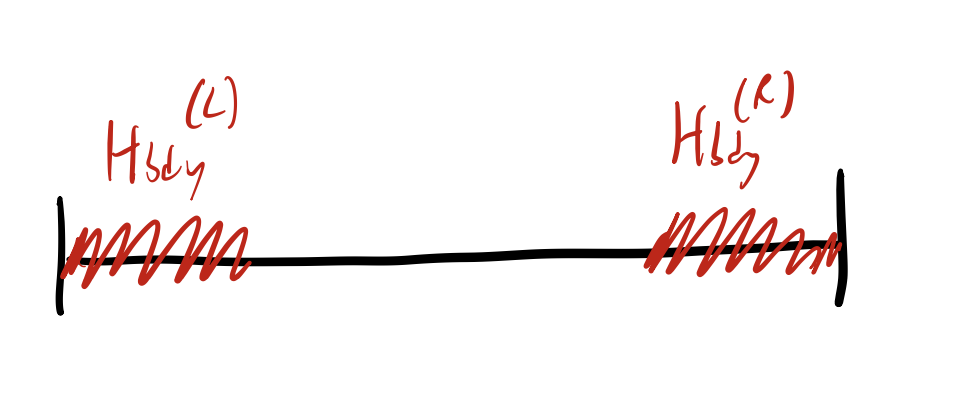
\includegraphics[scale=0.4]{Lectures/Images/lec14-boundaryH.png}
\end{center}

\subsection{Parametrizing the degenerate ground states}
Let's go back to the simple case with $H^{(L)}_{\text{bdy}} = H^{(R)}_{\text{bdy}} = 0$. Let's construct 4 ground states. Notice that $[Z_1, H] = [Z_{2N}, H] = 0$ because the terms at the boundary are $Z_1X_2Z_3$ and $Z_{2N-2}X_{2N-1}Z_{2N}$. The ground states correspond to states with $Z_1 = \pm 1$, $Z_{2N} = \pm 1$. The degrees of freedom at the ends of the chain are responsible for the degeneracy. It is as if there is an effective qubit at the right end of the chain and the left end of the chain. Let us define:
\begin{equation}
    \begin{split}
        \ket{\Omega, \uparrow\uparrow} &= \ket{\set{Z_{i-1}X_iZ_{i+1} = 1}, Z_1 = Z_{2N} = 1}
        \\ \ket{\Omega, \uparrow\downarrow} &= \ket{\set{Z_{i-1}X_iZ_{i+1} = 1}, Z_1 = 1, Z_{2N} = -1}
        \\ \ket{\Omega, \downarrow\uparrow} &= \ket{\set{Z_{i-1}X_iZ_{i+1} = 1}, Z_1 = -1, Z_{2N} = 1}
        \\ \ket{\Omega, \downarrow\downarrow} &= \ket{\set{Z_{i-1}X_iZ_{i+1} = 1}, Z_1 = Z_{2N} = -1}
    \end{split}
\end{equation}
We might be tempted to say that we have literally two qubits at the edge that are unentangled with the rest of the system, but this is not quite true. In order to understand these degrees of freedom at the edges, we will introduce the idea of a projective symmetry action.

\subsection{Projective symmetry action}
First, let us fix the relative phases of the 4 ground states. We notice that $Z_1, Z_{2N}$ commute with the Hamiltonian. But indeed there are two other operators that also commute with our Hamiltonian:
\begin{equation}
    [X_1Z_2, H] = [Z_{2N-1}X_{2N}, H] = 0
\end{equation}

\begin{center}
    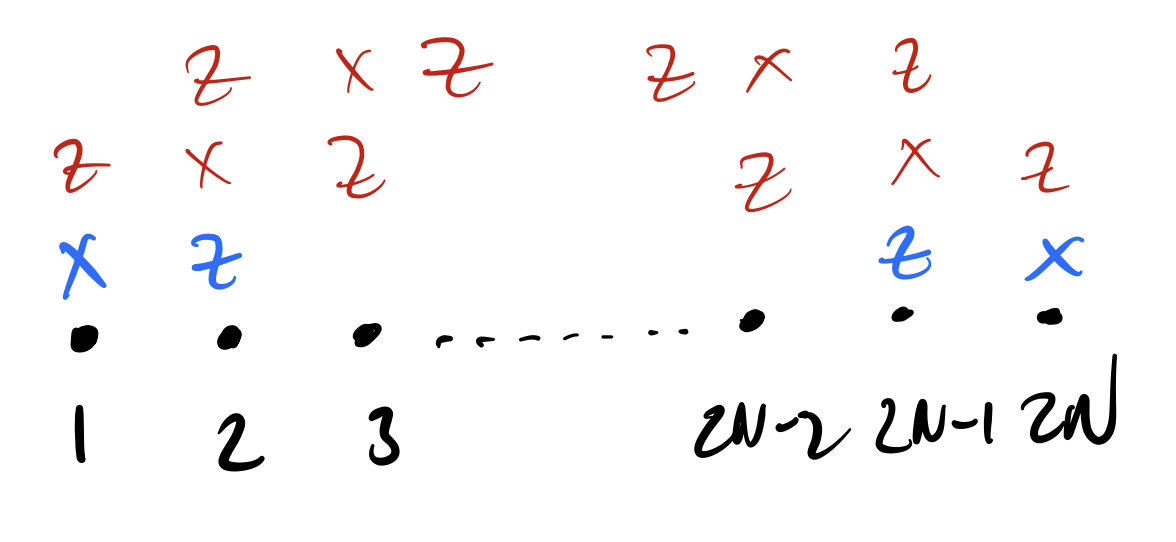
\includegraphics[scale=0.4]{Lectures/Images/lec14-boundaryterms.png}
\end{center}

Now note that $(X_1Z_2)Z_1 = -Z_1(X_1Z_2)$ and similarly $(Z_{2N-1}X_{2N})Z_{2N} = Z_{2N}(Z_{2N-1}X_{2N})$.

We can use $X_1Z_2$, $Z_{2N-1}X_{2N}$ to flip $Z_1, Z_{2N}$. This allows us to fix the relative phases, by using one of the ground states to define the other three:
\begin{equation}
    \begin{split}
        \ket{\Omega, \uparrow\downarrow} &= Z_{2N-1}X_{2N}\ket{\Omega, \uparrow\uparrow}
        \\ \ket{\Omega, \downarrow\uparrow} &= X_1Z_2\ket{\Omega, \uparrow\uparrow}
        \\ \ket{\Omega, \downarrow\downarrow} &= X_1Z_2Z_{2N-1}X_{2N}\ket{\Omega, \uparrow\uparrow}
    \end{split}
\end{equation}

Now that we have fixed the phases in this way, by construction $X_1Z_2$ acts as like a Pauli $X$ on the qubit degree of freedom on the left edge:
\begin{equation}
    \begin{split}
        X_1Z_2\ket{\Omega, \uparrow\uparrow} &= \ket{\Omega, \downarrow\uparrow}
        \\ X_1Z_2\ket{\Omega, \uparrow\downarrow} &= \ket{\Omega, \downarrow\downarrow}
        \\ X_1Z_2\ket{\Omega, \downarrow\uparrow} &= \ket{\Omega, \uparrow\uparrow}
        \\ X_1Z_2\ket{\Omega, \downarrow\downarrow} &= \ket{\Omega, \uparrow\downarrow}
    \end{split}
\end{equation}

Similarly, $Z_1$ acts like a pauli $Z$ on the qubit degree of freedom on the left:
\begin{equation}
    \begin{split}
        Z_1\ket{\Omega, \uparrow\uparrow} &= \ket{\Omega, \uparrow\uparrow}
        \\ Z_1\ket{\Omega, \uparrow\downarrow} &= \ket{\Omega, \uparrow\downarrow} 
        \\ Z_1\ket{\Omega, \downarrow\uparrow} &= -\ket{\Omega, \downarrow\uparrow}
        \\ Z_1\ket{\Omega, \downarrow\downarrow} &= -\ket{\Omega, \downarrow\downarrow}
    \end{split}
\end{equation}


We can now introduce some notation; the ground state action of $X_1Z_2 \leftrightarrow X^{(L)}$ and $Z_1 \leftrightarrow Z^{(L)}$. Identical relations/action happens on the right edge, where $Z_{2N-1}X_{2N} \leftrightarrow X^{(R)}$ and $Z_{2N} \leftrightarrow Z^{(R)}$ for the qubit degree of freedom on the right.

Now, let's compute the ground state action of $S_e, S_o$. Notice:
\begin{equation}
    S_e = X_2X_4\ldots X_{2N-2}X_{2N} = Z_1(Z_1X_2Z_3)(Z_3Z_4Z_5)\ldots (Z_{2N-3}X_{2N-2}Z_{2N-1})Z_{2N-1}X_{2N}
\end{equation}
What is nice about this product is all of the terms in the interior act like the identity on the ground states. Looking at the remaining operators on the boundaries, $Z_1$ acts like $Z^{(L)}$ and $Z_{2N-1}X_{2N}$ acts like $X^{(R)}$, so we conclude that the ground state action of $S_e$ is:
\begin{equation}
    S_e \cong Z^{(L)}X^{(R)}
\end{equation}
For $S_o$:
\begin{equation}
    S_o = X_1X_3X_5\ldots X_{2N-3}X_{2N-1} = X_1Z_2(Z_2X_3Z_4)(Z_4X_5Z_6)\ldots (Z_{2N-4}X_{2N-3}Z_{2N-2})(Z_{2N-2}X_{2N-1}Z_{2N})Z_{2N}
\end{equation}
and so:
\begin{equation}
    S_o \cong X^{(L)}Z^{(R)}
\end{equation}
We now know how the symmetries act on the 4-d subspace. Let us write:
\begin{equation}
    S_e = S_e^{(L)} \otimes S_e^{(R)} = Z^{(L)}\otimes X^{(R)}
\end{equation}
\begin{equation}
    S_o = S_o^{(L)} \otimes S_o^{(R)} = X^{(L)}\otimes Z^{(R)}
\end{equation}
We can already see something interesting here. Notice that $S_eS_o = S_oS_e$. We can see this because they have anticommutation on both edges (so the total operator commutes). Of course we could see this from the original form of hte symmetry operators as well. But the key observation is that:
\begin{equation}
    S_e^{(L)}S_o^{(L)} = -S_o^{(L)}S_e^{(L)}
\end{equation}
\begin{equation}
    S_e^{(R)}S_o^{(R)} = -S_o^{(R)}S_e^{(R)}
\end{equation}
Thus, the qubits on the left/right ends of the chain transform under a projective representation of $\mathbb{Z}_2 \times \mathbb{Z}_2$.

A projective representation is a presentation where group relations are obeyed up to a phase. In a linear representation (what you may be used to), for two representations of group elements $g, h$ we have:
\begin{equation}
    U^g U^h = U^{gh}
\end{equation}
for a projective representation, we have that the representations multiply up to a phase $\omega(g, h)$:
\begin{equation}
    U^g U^h = \omega(g, h)U^{gh}
\end{equation}

As a concrete example, let's look at the spin-1/2 representation of $SO(3)$:
\begin{equation}
    U(R_{\zhat}(\pi))^2 = -\II
\end{equation}

Also, note that there is a case of a special projective representation. If the phases follow the relation:
\begin{equation}
    U^g U^h = U^{gh}\frac{\nu(g)\nu(h)}{\nu(gh)}
\end{equation}
then we can redefine:
\begin{equation}
    \tilde{U}^g = \frac{U^g}{\nu(g)}
\end{equation}
which makes the projective representation a linear one:
\begin{equation}
    \tilde{U}^g\tilde{U}^h = \tilde{U}^{gh}
\end{equation}

However note that what we have here is a non-trivial projective representation, because changing the phase of the operators does not change the commutation relations of the operators. This is a key feature of SPT phases; the projective representation cannot be lifted.

Another remark; classifying SPTs is the same as classifying projective representations, i.e. the possible $\omega$s, which are given by the cohomology group $H^2(G, U(1))$. For higher dimensions, this roughly generalizes to $H^3(G, U(1))$.

A very general feature of SPT phases defined on an open chain is that we find that the ground state space $V$ breaks up into $V = V^{(L)} \otimes V^{(R)}$ (here the left/right Hilbert spaces are 2-d, but this can generalize). We can similarly break up the symmetry group into $U^g = U^g_L \otimes U^g_R$.